\documentclass[aspectratio=169,unicode,compress,14pt]{beamer}
\usepackage{luatexja-preset,amsmath,ulem,tikz,here,color}
\usetikzlibrary{shapes,snakes,arrows.meta,positioning,calc}
\def\nodecolor{blue!20}%
\input{../template/beamertemp.tex}
\input{../template/mylisting.tex}
\setmonofont{Meslo LG L}
\setsansfont{Source Han Sans JP}
\setromanfont{Takao Ex Mincho}
\renewcommand{\familydefault}{\rmdefault}
\setbeamersize{text margin left=1\zw}
\setbeamersize{text margin right=1\zw}
\newlength{\bitlen}
\title{Optimizing Lua VM Bytecode using Data Flow Analysis}
\institute{情報特別演習 報告会}
\keywords{Lua VM, Register-based VM, optimization}
\author{Satoru Kawahara}
\lstset{numbers=none}
\begin{document}
\maketitle
\section{motivation}
\begin{frame}[fragile]
\frametitlesec
\alert{Lua VM}, register-based Virtual Machine
\begin{figure}[H]
	\bgroup
	\footnotesize\tt
	\tikzset{
		LL/.style={
			draw=black,decorate,
			decoration={snake, segment length=3mm,post}
		},
		every node/.style = {draw, align=center}
	}

	\begin{tikzpicture}
		\node[ellipse,fill=\nodecolor] (source) {Lua source};
		\node[right = 2 of source, ellipse,fill=\nodecolor] (bytecode) {\textcolor<2>{red}{bytecode}};
		\node[draw=none, above] at ($(source)!0.5!(bytecode)$) {\textrm{compile}};
		\node[draw=none,right = of bytecode] (run) {(run on the VM)};
		\draw[->] (source) -- (bytecode);
		\draw[->] (bytecode) -- (run);
	\end{tikzpicture}
	\egroup
\end{figure}
\pause
\pause

積極的に最適化が\structure{行われない}

\bgroup
\small
\begin{minipage}{.1\textwidth}
\ 
\end{minipage}
\begin{minipage}{.3\textwidth}
\begin{lstlisting}[language={[5.3]lua}]
local x = 3
local y = 5
print(x + y)\end{lstlisting}
\end{minipage}
\begin{minipage}{.2\textwidth}
\begin{center}
\structure{$\Rightarrow$}

compile
\end{center}
\end{minipage}
\begin{minipage}{.35\textwidth}
	\begin{lstlisting}
LOADK       0   0
LOADK       1   1
GETTABUP   2    0   -3
ADD         3   0    1
CALL        2   2    1
RETURN      0   1\end{lstlisting}
\end{minipage}
\begin{minipage}{.1\textwidth}
\ 
\end{minipage}
\egroup

\only<4->{%
\vskip-3.3\zw%
\hspace{10\zw}%
\fcolorbox{black}{white}{\parbox{\dimexpr10\zw\fboxsep-2\fboxrule\relax}{\alert{コンパイル時に値が\ \ $\uparrow$ 分かる(定数化可能)}}}%
\vskip.4\zw%
}

\only<5->{%
\vskip-8.5\zw%
\hskip7.7\zw%
\fcolorbox{black}{white}{\parbox{\dimexpr11\zw\fboxsep-2\fboxrule\relax}{\alert{足し算の結果が分かればこの定数はいらない\ \ $\rightarrow$}}}%
\vskip5.7\zw%
}
\end{frame}


\section{summary}
\begin{frame}[fragile]
\frametitlesec
\begin{figure}[H]
	\centering
	\bgroup
	\footnotesize\tt
	\tikzset{
		LL/.style={
			draw=black,decorate,
			decoration={snake, segment length=3mm,post}
		},
		>={Latex[width=1mm,length=1mm]},
		every node/.style = {draw, align=center},
	}

	\newcommand{\byty}{-1.3}

	\begin{tikzpicture}
		\node[ellipse,fill=\nodecolor] (source) at (5.3, 3.2) {\textsf{Source}};
		\node[above = of source,star,star points=6,star point ratio=0.8,fill=\nodecolor] (bytecode) {\textsf{bytecode}};
		\coordinate[above = of bytecode] (pt9);
		\coordinate[right = 3.7 of pt9] (pt5);
		\node[rectangle,fill=\nodecolor,below = 0.4 of pt5] (adata) {analyzed data};
		\node[rectangle,text width=3.6cm,align=center,fill=\nodecolor,below = 2 of adata] (cfgduch) {\alert<2>{Control Flow Graph\\\& DU~Chain}};
		\coordinate[right = 4.3 of adata] (pt6);
		\coordinate[right = 2 of adata] (pt7);
		\coordinate[right = 2 of cfgduch] (pt8);
		\draw[->] (source) -- (bytecode);
		\draw (bytecode) -- (pt9);
		\draw[->] (pt9) -| (adata);
		\draw[->] (adata) -- (cfgduch);
		% \draw[LL,thick,>=latex] (adata) -- (pt7);
		% \draw[LL,thick,>=latex] (cfgduch) -- (pt8);
		\node[fill=yellow!20,rectangle, text width=19\zw,below = -1.6\zw of pt6] (opts){%
			\textcolor{red}{optimizer}\\%
			\begin{itemize}
				\item constant folding
				\item constant propagation
				\item dead-code elimination
				\item function inlining
				\item unreachable block removal
				\item unused resources removal
			\end{itemize}};
		\draw[LL,thick,>=latex,->] (adata) -- (opts);
		\draw[LL,thick,>=latex,->] (cfgduch) -- (opts);
		\coordinate[below = 1.3 of opts] (pt2);
		\coordinate[left = 8 of pt2] (pt3);
		\draw[to path = {-| (\tikztotarget)},->] (opts) |- (pt3) |- (adata);
		% \node[draw=none, above] at ($(pt2)!0.5!(pt3)$) {again};
		\node[right = 1.3 of pt2,text width=4.8em,fill=\nodecolor,circle] (optbc) {\textsf{optimized\\bytecode}};
		\draw[->] (pt2) --  (optbc);
	\end{tikzpicture}
	\egroup
\end{figure}
% TODO: data flow analysisな部分を赤枠で囲って、横にCFGを置くなどするといいかも
\end{frame}

\subsection{Bytecode}
\begin{frame}
	\frametitlesubs
	\begin{figure}
		\centering
		\begin{tikzpicture}
			\node[text width=13\zw] (sousa) at (0, 0) {Lua VM 5.3のバイトコード\\を操作したい};
			\node[right = .5 of sousa] (arrow) {$\Rightarrow$};
			\node[right = .5 of arrow, text width=13\zw] {バイトコードのdocumentは\\\alert<2->{ない}};
		\end{tikzpicture}
	\end{figure}

	\pause
	\vspace{3\zw}
	\begin{center}
		$\Rightarrow$ \alert{自分で読み解くしかない}
	\end{center}
\end{frame}
\begin{frame}
	\frametitlesubs

	有志の非公式ドキュメント
	\begin{itemize}
		\item Lua VM 5.3 instructions (bytecodeではない)\footnote{\url{https://github.com/dibyendumajumdar/ravi/blob/master/readthedocs/lua_bytecode_reference.rst}}
		\item Lua VM 5.1 reference\footnote{\url{http://luaforge.net/docman/83/98/ANoFrillsIntroToLua51VMInstructions.pdf}}
	\end{itemize}
	\pause

	Lua VM bytecodeを読むためのツール
	\begin{itemize}
		\item \lstinline{luac -l -l luac.out}
		\item \lstinline{xxd -g 1 luac.out | nvim - -R}\pause
		\item ソースコード\footnote{\url{https://www.lua.org/source}}
	\end{itemize}

	\pause
	\begin{center}
		簡単に言うと\alert{\Huge{}気合}
	\end{center}
\end{frame}
\begin{frame}[fragile]
	\frametitlesubs
	\hspace{-.5\zw}
	\begin{minipage}[t]{.34\textwidth}
		\bgroup\footnotesize
		\begin{lstlisting}[numbers=none,language={[5.3]lua}]
print("hello, world!")
		\end{lstlisting}
		\tiny
		\begin{lstlisting}[numbers=none]
 $ luac -l -l luac.out

main <hello.lua:0,0> (4 instructions at 0x16e79e0)
0+ params, 2 slots, 1 upvalue, 0 locals, 2 constants, 0 functions
  1  [1]  GETTABUP     0 0 -1  ; _ENV "print"
  2  [1]  LOADK        1 -2    ; "hello, world!"
  3  [1]  CALL         0 2 1
  4  [1]  RETURN       0 1
constants (2) for 0x16e79e0:
  1  "print"
  2  "hello, world!"
locals (0) for 0x16e79e0:
upvalues (1) for 0x16e79e0:
  0  _ENV    1       0
		\end{lstlisting}
		\egroup
	\end{minipage}
	\begin{minipage}{.01\textwidth}
		\ 
	\end{minipage}
	\begin{minipage}[t]{.64\textwidth}
		\pause
		\bgroup\tiny
		\begin{lstlisting}[numbers=none]
$ xxd -g 1 luac.out
00000000: 1b 4c 75 61 53 00 19 93 0d 0a 1a 0a 04 08 04 08  .LuaS...........
00000010: 08 78 56 00 00 00 00 00 00 00 00 00 00 00 28 77  .xV...........(w
00000020: 40 01 0b 40 68 65 6c 6c 6f 2e 6c 75 61 00 00 00  @..@hello.lua...
00000030: 00 00 00 00 00 00 02 02 04 00 00 00 06 00 40 00  ..............@.
00000040: 41 40 00 00 24 40 00 01 26 00 80 00 02 00 00 00  A@..$@..&.......
00000050: 04 06 70 72 69 6e 74 04 0e 68 65 6c 6c 6f 2c 20  ..print..hello,
00000060: 77 6f 72 6c 64 21 01 00 00 00 01 00 00 00 00 00  world!..........
00000070: 04 00 00 00 01 00 00 00 01 00 00 00 01 00 00 00  ................
00000080: 01 00 00 00 00 00 00 00 01 00 00 00 05 5f 45 4e  ............._EN
00000090: 56                                                                  V
		\end{lstlisting}
		\egroup\normalfont
		\pause
		\begin{center}
			\vspace{1\zw}
			\LARGE
			\alert{???}
		\end{center}
	\end{minipage}
\end{frame}
\begin{frame}[fragile]
	\frametitlesubs
	\begin{center}
		\begin{minipage}[t]{.4\textwidth}
			\bgroup\tiny
			\begin{lstlisting}[numbers=none]
1b 4c 75 61 53 00 19 93 0d 0a 1a 0a 04 08 04 08
08 78 56 00 00 00 00 00 00 00 00 00 00 00 28 77
40 01 0b 40 68 65 6c 6c 6f 2e 6c 75 61 00 00 00
00 00 00 00 00 00 02 02 04 00 00 00 06 00 40 00
41 40 00 00 24 40 00 01 26 00 80 00 02 00 00 00
04 06 70 72 69 6e 74 04 0e 68 65 6c 6c 6f 2c 20
77 6f 72 6c 64 21 01 00 00 00 01 00 00 00 00 00
04 00 00 00 01 00 00 00 01 00 00 00 01 00 00 00
01 00 00 00 00 00 00 00 01 00 00 00 05 5f 45 4e
56
			\end{lstlisting}
			\egroup
		\end{minipage}
	\end{center}
	\pause
	\begin{figure}[h]
		\def\position{(0.1, -1.76)}
		\tikzset{just here/.style = {above right,inner sep=0mm}}
		\centering
		\begin{tikzpicture}[remember picture]
			\useasboundingbox (0.1,-1.76);
			\coordinate (top) at (-3, 2.3);
			\node[above right = .2 of top] (label) {\textcolor{blue}{header block}};
			\coordinate[right = 6.2 of top] (p1);
			\coordinate[below = 0.55 of p1] (p2);
			\coordinate[left = 5.4 of p2] (p3);
			\coordinate[below = 0.28 of p3] (p4);
			\coordinate[left = 0.8 of p4] (p5);
			\draw[blue, dashed, very thick] (top) -- (p1) -- (p2) -- (p3) -- (p4) -- (p5) -- (top);
		\end{tikzpicture}
	\end{figure}
	\pause
	\begin{figure}[h]
		\tikzset{just here/.style = {above right,inner sep=0mm}}
		\centering
		\begin{tikzpicture}[remember picture]
			\useasboundingbox (0.1,-1.76);
			\coordinate (bottom) at (-3, 1.33);
			\node[below right = .2 of bottom] (label) {\textcolor{red}{function block}};
			\coordinate[right = 6.2 of bottom] (p1);
			\coordinate[above = 2.14 of p1] (p2);
			\coordinate[left = 5.4 of p2] (p3);
			\coordinate[below = .28 of p3] (p4);
			\coordinate[left = .8 of p4] (p5);
			\draw[red, dashed, very thick] (bottom) -- (p1) -- (p2) -- (p3) -- (p4) -- (p5) -- (bottom);
		\end{tikzpicture}
	\end{figure}
\end{frame}


\section{optimize}
% \begin{frame}
% \frametitlesec

% \begin{figure}[H]
	% \bgroup
	% \small\tt
	% \tikzset{
		% LL/.style={
			% draw=black,decorate,
			% decoration={snake, segment length=3mm,post}
		% },
		% every node/.style = {draw, align=center}
	% }

	% \begin{tikzpicture}
		% \node[star,star points=6,star point ratio=0.8,fill=\nodecolor] (source) {bytecode};
		% \node[right = 2 of source, ellipse,fill=\nodecolor] (tformat) {\alert<2>{treatable format}};
		% \draw[->] (source) -- (tformat);
		% \coordinate[below = 2 of tformat] (pt1) {};
		% \node[left = 2 of pt1,fill=\nodecolor] (cfg) {\alert<3->{Control Flow Graph}};
		% \node[below = of cfg,fill=\nodecolor] (duchain) {\alert<3->{Define-Use Chain}};
		% \draw[->] (tformat) -- (cfg);
		% \draw[->] (cfg) -- (duchain);
		% \node[below = .5 of pt1,fill=yellow!20] (opts) {optimizer};
		% \draw[->] (cfg) -- (opts);
		% \draw[->] (duchain) -- (opts);
	% \end{tikzpicture}
	% \egroup
% \end{figure}
% \end{frame}
\subsection{Control Flow Graph \& Define-Use Chain}
\begin{frame}[fragile]
\frametitlesubs
\begin{minipage}{.23\textwidth}
	\scriptsize
	\begin{lstlisting}[language={[5.3]lua}]
local b = true

if b then
	print("hello")
else
	print"world"
end
\end{lstlisting}

\pause
\vspace{-2\zw}
\begin{center}
	\normalsize
\noindent$\Downarrow$
\end{center}
\vspace{-2\zw}
\begin{lstlisting}
LOADBOOL      0   1    0
TEST          0   0 
JMP           0   4 
GETTABUP      1   0   -1
LOADK         2   1 
CALL          1   2    1
JMP           0   3 
GETTABUP      1   0   -1
LOADK         2   2 
CALL          1   2    1
RETURN        0   1 
\end{lstlisting}
\end{minipage}\pause
\begin{minipage}{.06\textwidth}
\begin{flushright}
	\ $\Rightarrow$
\end{flushright}
\end{minipage}
\begin{minipage}{.56\textwidth}
	\begin{figure}[h]
	\centering
	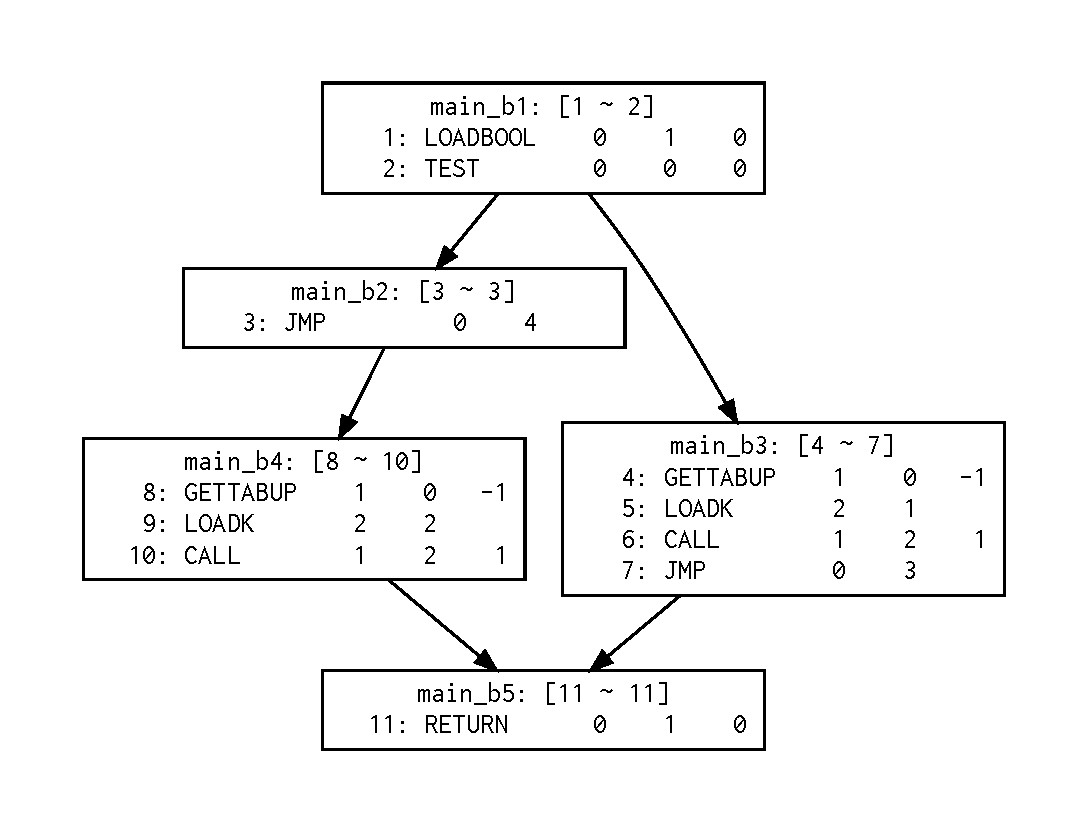
\includegraphics[width=1.3\textwidth]{figure/cfg.pdf}
	\end{figure}
\end{minipage}
\end{frame}
\subsection{optimize}
% \TableOfContents{currentsection}
\begin{frame}
\frametitlesec
以下の最適化を可能な限り何度もおこなう
\begin{itemize}
	\item constant folding (定数畳み込み)
	\item constant propagation (定数伝播)
	\item dead-code elimination (不要式の削除)
	\item function inlining (関数展開)
	\item unreachable block removal (到達不可能なブロックの削除)
	\item unused resources removal (不要資源の削除)
\end{itemize}
\end{frame}


\section{benchmark}
% \subsection{Linpack benchmark}
% \begin{frame}[fragile]
% \frametitlesubs
% Linpack benchmark\footnote{\url{https://www.jasondavies.com/optimising-lua/JasonDaviesDissertation.pdf}にあるソースコードを利用}
% \end{frame}
% \subsection{function inlining}
\begin{frame}[fragile]
\frametitlesec
\begin{minipage}{.05\textwidth}
	\ 
\end{minipage}
\begin{minipage}[t]{.3\textwidth}
	\scriptsize
	\begin{lstlisting}[language={[5.3]lua}]
local function pow(i)
	return i * i
end

local a = {}

for i = 1, 10000000 do
	a[i] = pow(i)
end
	\end{lstlisting}
	\begin{minipage}[t]{1.2\textwidth}
		% \begin{center}
			\vspace{3\zw}
			\only<6>{\Large\alert{1.4倍の高速化}}
		% \end{center}
	\end{minipage}
\end{minipage}
\begin{minipage}[t]{.2\textwidth}
	\pause
	\vspace{3\zw}
	\ \ \ \ \ \ \ $\Rightarrow$

	\vspace{6\zw}
	\only<6>{\ \ \ \ \ \ \ $\Leftarrow$}
\end{minipage}
\begin{minipage}[t]{.3\textwidth}
	\bgroup
	\scriptsize
	\begin{lstlisting}[style=snippet,escapechar={@}]
......
FORPREP         2 4    
@\color<5>{brown}{MOVE\ \ \ \ \ \ \ \ 6\ 0}@
MOVE            7 5
@\alert<4>{CALL\ \ \ \ \ \ \ \ 6\ 2\ 2}@
SETTABLE        1 5 6
FORLOOP         2 -5   
......
	\end{lstlisting}
	\egroup

	\pause
	\vspace{-1\zw}
	\begin{center}
		$\Downarrow$
	\end{center}
	\vspace{-1\zw}
	\scriptsize
	\begin{lstlisting}[style=snippet,escapechar={@}]
......
FORPREP         2 4    
MOVE            7 5
@\alert<4>{MUL\ \ \ \ \ \ \ \ \ 8\ 7\ 7}@
@\alert<4>{MOVE\ \ \ \ \ \ \ \ 6\ 8}@
SETTABLE        1 5 6
FORLOOP         2 -5   
......
	\end{lstlisting}
\end{minipage}
\end{frame}


\section{まとめ}
\begin{frame}
    \frametitlesec

    \begin{itemize}
        \item[\coloremoji{🌋}] Algebraic Effectsが楽しい

            ICFP 2018やML Workshop2018にも\\
            AE関連のトピック%
            \footnote{\url{https://icfp18.sigplan.org/event/mlfamilyworkshop-2018-papers-programming-with-abstract-algebraic-effects}}%
            \footnote{\url{https://icfp18.sigplan.org/event/icfp-2018-papers-versatile-event-correlation-with-algebraic-effects}}

        \item[\coloremoji{🉐}] Algebraic Effects使おう

            \begin{itemize}
                \item[\coloremoji{🛠}] インプリいろいろ
                \item[\coloremoji{💪}] なければ自作も可
            \end{itemize}

        \item[\coloremoji{👨‍💻}] 研究やってます
    \end{itemize}
\end{frame}


\end{document}
